\section{What the learned ranking and safety mask contribute}
\label{sec:jesper-components}
\contributionauthor{Jesper Eggers}
The aggregate outcomes suggest benefits from both constraints and learned
selection. We now quantify their separate deployment effects and whether
those effects interact. The four configurations form a controlled $2\times2$ deployment experiment.
Writing $\mu_{q,m}$ for mean official score under ranking rule $q$ and
mask $m$, the temporal mask's effect with the learned network is
$\Delta_{\mathrm{Q}}=\mu_{\mathrm{Q,T}}-\mu_{\mathrm{Q,R}}$.
Its effect under uniform action selection is
$\Delta_{\mathrm{random}}=\mu_{\mathrm{random,T}}-\mu_{\mathrm{random,R}}$.
The difference $I=\Delta_{\mathrm{Q}}-\Delta_{\mathrm{random}}$ tests whether
the mask's measured effect depends on the ranking rule. We resample the
four results for each seed together to preserve the paired design.
The interaction captures their joint operation: filtering actions changes
the preference expressed and the subsequent trajectory.

For learned selection, replacing the RUEHL mask with the temporal implementation adds
1.375 points [1.090, 1.670] against rule-based opponents and 2.135
[1.775, 2.505] against the mixed population. Self-destruction decreases
by 36.5 and 54.0 percentage points, respectively. The random controls
also benefit: their score gains are 0.940 [0.715, 1.185] and 0.985
[0.760, 1.230]. This supports a deployment benefit from the temporal-mask implementation
even under random ranking.

The score interaction is 0.435 [0.075, 0.805] for rule-based opponents
and 1.150 [0.715, 1.600] for mixed opponents. In both populations, the
observed temporal-mask benefit is larger with learned selection. The
components therefore complement each other in this experiment, although
the smaller interaction's interval approaches zero and remains a
pointwise, exploratory comparison.

Within a fixed mask, learned-versus-random selection measures the deployed
value of trained preferences. Masked random controls retain legality,
danger, and bomb-usefulness checks. An advantage over them demonstrates
value beyond these constraints, without implying that the network learned
the safety rules independently. Random deployment does not recreate an
otherwise identical agent trained without learning.

The frozen network was trained with the temporal mask. Swapping to RUEHL's
mask changes both its immediate choice set and the states subsequently
encountered. Distribution shift is therefore part of the tested deployment
intervention, rather than a nuisance removed by holding weights fixed.
The paired contrast supports a causal statement about this implementation
under these opponents; it cannot establish the performance of RUEHL's
own trained network or the sample efficiency of either mask during
training. A stronger learning claim requires matched retraining budgets,
representations, rewards, and multiple initialization seeds.

\begin{figure}[!htbp]
\centering
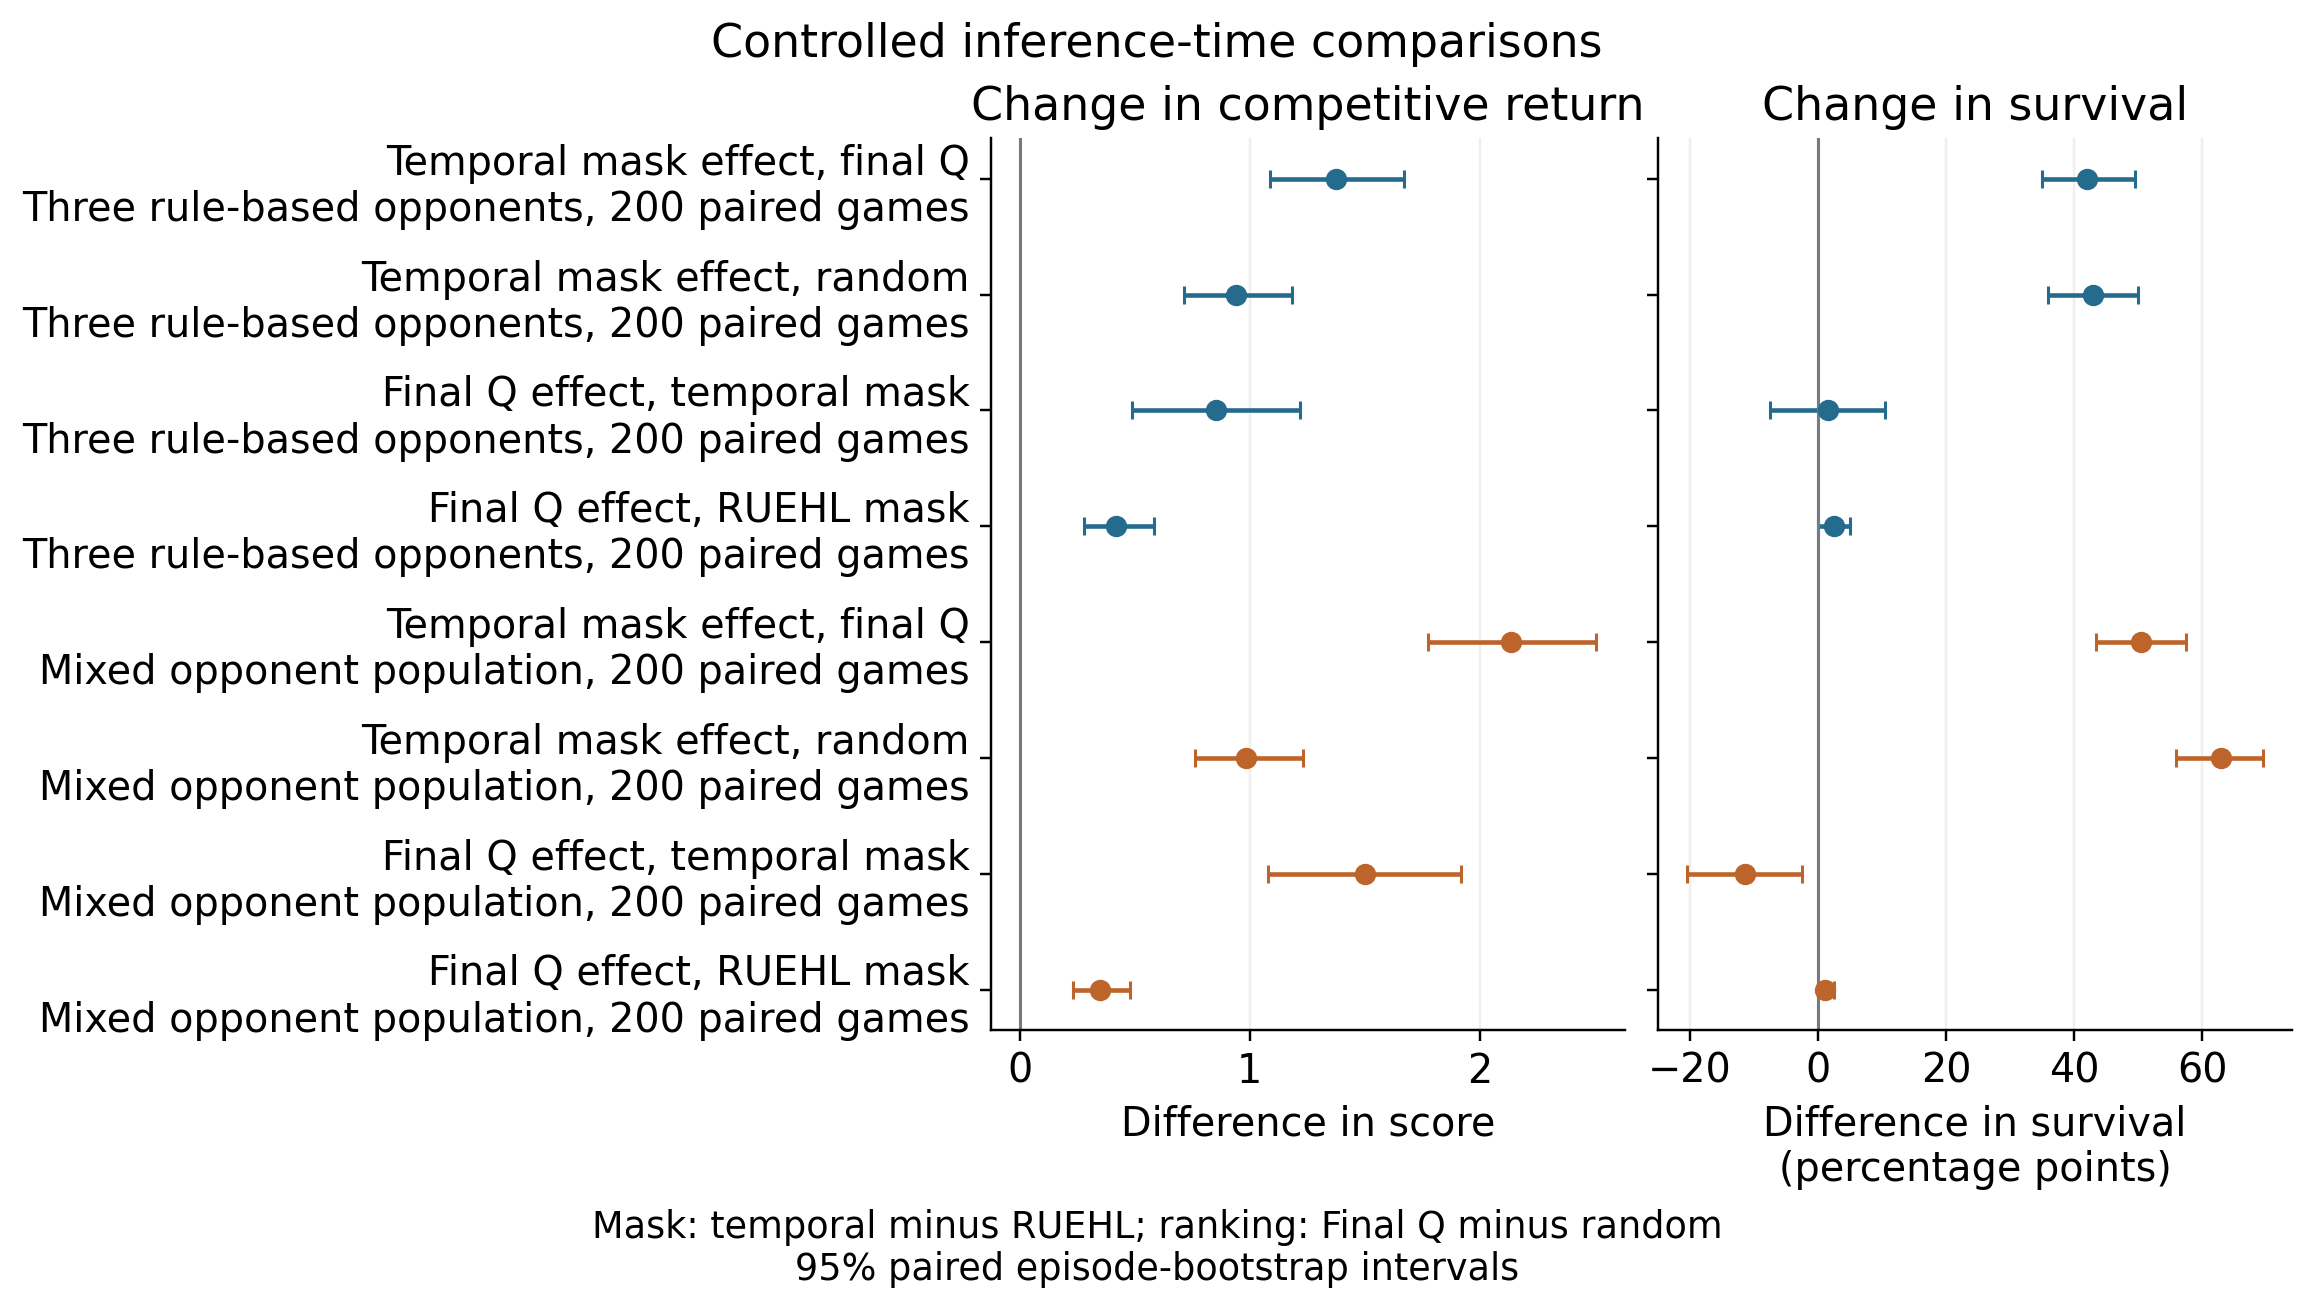
\includegraphics[width=\textwidth]{figures/frozen_evaluation_components.png}
\caption{Paired deployment effects on score and survival. Mask effects subtract
RUEHL from temporal masking; ranking effects subtract uniform random from
Final Q selection within a fixed mask. Whole seed-matched episodes are
resampled together.}
\label{fig:jesper-components}
\end{figure}
\FloatBarrier
